\documentclass[12pt]{article}
%\input{hw_macros.tex}

\setlength{\topmargin}{-.75in} \addtolength{\textheight}{2.00in}
\setlength{\oddsidemargin}{.00in} \addtolength{\textwidth}{.75in}

\usepackage{amsmath,color,amssymb,graphicx,esdiff}
\usepackage[shortlabels]{enumitem}
\pagestyle{empty}
\usepackage{listings}

\setlength{\parindent}{0in}
\setlist[enumerate]{leftmargin=*}
\begin{document}

{\sc {\bf {\large Homework 1}}
            \hfill {MTH 629, Fall 2021}}
\bigskip

{\bf Due Wed. Sept. 15\textsuperscript{th} by 11:59 pm on Canvas}

\section{Chapter 1}

\textbf{Problem 1.}
Given the following survival time data (in weeks) for $n = 15$ subjects,
$$
1+, 2, 2, 2+, 2+, 3, 3, 3, 3+, 4+, 4+, 5, 5, 7, 8+
$$ where $+$ denotes right censored data, complete the following table:

\begin{center}
\begin{tabular}{ c c c c }
 $t_{(f)}$ & $m_{f}$ & $q_{f}$ & $R(t_{(f)})$ \\
 \hline \\
 $0$ & $?$ & $?$ & $15$ \\
 $2$ &?  &?  &? \\
 $3$ &?  &?  &? \\
 $5$ &?  &?  &? \\
 $7$ &?  &?  &?
\end{tabular}
\end{center}

\begin{enumerate}
\item Fill in the missing entries in the table.
\item Use the table to estimate the following five probabilities
\[
P(T>t_{(f)}|T \ge t_{(f)}) \text{ for } t=0,2,4,5,7.
\]
\item Compute the average survival time ($\overline{T}$) and the average hazard rate ($\overline{h}$).
\end{enumerate}


\textbf{Problem 2.}
Consider the comparison of the following survival curves for groups $A, B$ and $C$.
\begin{center}
 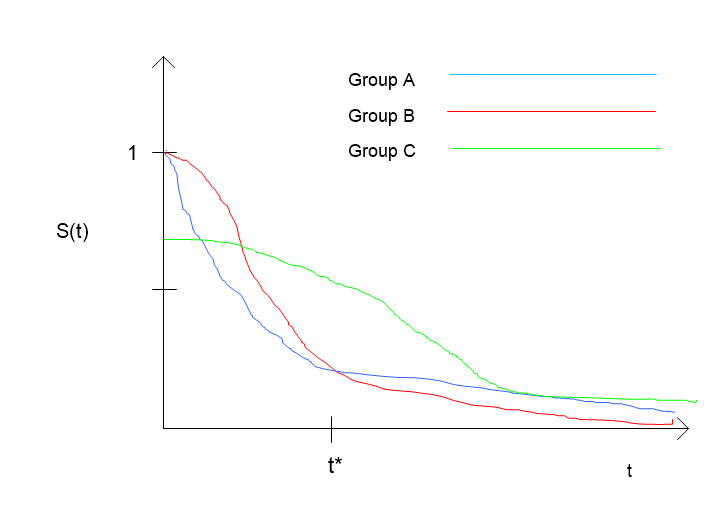
\includegraphics[width = \textwidth]{Chpt1_surv}
 \end{center}
\begin{enumerate}
\item Which group has the worst survival prognosis before time $t^*$?
\item Which group has a best survival prognosis after time $t^*$?
\item Which group has the longest median survival time?
\end{enumerate}

\textbf{Problem 3.}
Survival times (in years) are given for two study groups, each with $25$ participants. Group 1 has no history of chronic disease (CHR $= 0$), and group 2 has a positive history of chronic disease (CHR $= 1$): \\

Group 1 (CHR $= 0$): 11.3+, 6.4, 8.5, 13.7+, 10.1, 10.0, 5.7, 8.2, 2.0, 12.0, 9.9, 13.6+, 8.8, 2.2, 1.6, 10.2, 10.7, 11.1+, 5.3, 2.5, 10.6, 2.5, 5.7, 4.8, 2.7 \\

Group 2 (CHR $= 1$): 4.8, 2.9, 10.7, 9.3, 9.1, 3.9, 5.0, 1.2, 4.4, 12.0, 2.9, 1.2, 6.9, 1.4, 3.0, 3.9, 3.5, 6.5, 9.9, 3.6, 5.2, 9.8, 6.8, 4.7, 3.9 \\

\begin{itemize}
	\item[(a)] Complete the following survival tables  for both Group 1 and Group 2: \\

\begin{center}
\begin{tabular}{ c c c c c }
 & $t_{(f)}$ & $m_{f}$ & $q_{f}$ & $R(t_{(f)})$ \\
 \hline \\
 Group 1: & $0.0$ & $0$ & $0$ & $25$ persons survive $\geq 0$ weeks \\
 & $1.6$ &1  &0  & $25$ persons survive $\geq 1.6$ weeks \\
 & $\vdots$ & $\vdots$ & $\vdots$ & $\vdots$
\end{tabular}
\end{center}

\begin{center}
\begin{tabular}{ c c c c c }
 & $t_{(f)}$ & $m_{f}$ & $q_{f}$ & $R(t_{(f)})$ \\
 \hline \\
 Group 2: & $0.0$ & $0$ & $0$ & $25$ persons survive $\geq 0$ weeks \\
 & $1.2$ &2  &0  & $25$ persons survive $\geq 1.2$ weeks \\
 & $\vdots$ & $\vdots$ & $\vdots$ & $\vdots$
\end{tabular}
\end{center}

	
	\item[(b)] Compute the average survival time ($\overline{T}$) and the average hazard rate ($\overline{h}$) for each group.
	
	\item[(c)] Based on the your answer in b), briefly explain which group has better overall survival prospects. What might be the problem with your argument?
\end{itemize}

\textbf{Problem 4.}
Give your own example of each of the following types of censoring:
\begin{enumerate}
\item Right Censoring:
\item Left Censoring:
\item Interval Censoring:
\end{enumerate}
\newpage
\textbf{Problem 5.}
\begin{enumerate}
\item
Identify the issue presented in each of the following studies as confounding or interaction. Then discuss how each of these issues might be dealt with in a statistical model.
\begin{enumerate}
\item A statistician working for ACME corporation collects data from male and female employees to see if there is a difference in the time it takes for new male and female employees to pass ACME Corp's programming certification. ACME Corp tends to hire male employees from technical colleges where students get several years of programming experience and female employees from liberal arts programs where students get at most one year of programming experience.
\item  A statistician working for ACME corporation collects data from male and female employees to see if there is a difference in the time it takes for male and female employees to pass ACME Corp's English Proficiency Exam (EPE). Older male employees tend to take more time to pass the EPE than female employees and younger male employees tend to take less time to pass the EPE than female employees.
\end{enumerate}
\item Present your own examples of confounding and interaction.
\end{enumerate}

\textbf{Problem 6.}
A group of 2000 patients are given different types of heart stents from Advanced Bionics and Juno Devices. A study is conducted concerning time, $T$, until major heart failure or death. Their survival information collected is given below:
\begin{center}
\textbf{Advanced Bionics}
\begin{tabular}{ c c c c }
 Time & \# at risk & \# events & \# survived \\ \hline
 0-10 yrs & 600 & 80 & 520 \\
 10–20 yrs &  400 & 280 & 120
\end{tabular} \\
120 left study at the end of 10 years
\end{center}
\begin{center}
\textbf{Juno Devices}
\begin{tabular}{ c c c c }
 Time & \# at risk & \# events & \# survived \\ \hline
 0-10 yrs & 400 & 100 & 300 \\
 10–20 yrs &  250 & 150 & 100
\end{tabular} \\
50 left study at the end of 10 years.
\end{center}
Based on the information above, and assuming independent censoring, summarize the 10 and 20 year survival experiences of the two groups.

\newpage
\textbf{Problem 7.}
Given the pdfs below find the survival ($S(t)$) and hazard function (h(t)). Use the fact that
\[
S(t) = P(T>t) = \int_t^{\infty} f(u) du.
\]

\begin{itemize}
	\item[(a)]
	$$
	f(t) = \begin{cases} \frac{3}{2} (\frac{t}{2})^2 \exp[-(\frac{t}{2})^3], &t > 0 \\
		0, &t \leq 0.
		\end{cases}
	$$
	\item[(b)] Use integration by parts.
	$$
	f(t) = \begin{cases} (1/9)t\exp(-t/3), &t > 0 \\
		0, &t \leq 0.
		\end{cases}
    $$
    \item[(c)] After you find the hazard function, identify a type of survival population that might have such a hazard.
    $$
	f(t) = \begin{cases} \frac{18}{(t+3)^3}, &t > 0 \\
		0, &t \leq 0.
		\end{cases}
    $$
\end{itemize}

\section{Chapter 2}

\textbf{Problem 1.} Multiple myeloma is a malignant disease characterised by the accumulation
of abnormal plasma cells, a type of white blood cell, in the bone marrow. Unless
treated, the condition is invariably fatal. The aim of a study carried out at
the Medical Center of the University of West Virginia, USA, was to examine the association between the values of certain explanatory variables or covariates and the survival time of patients. In the study, the primary response
variable was the time, in months, from diagnosis until death from multiple
myeloma.
\begin{enumerate}[(a)]
\item Load the data by using the following command in R:

\bigotimes

\item Patients are placed in  two types of treatment facilities: the myelmoa clinic at the City Hospital (coded as Clinic=1) and the private research clinic at the University (coded as Clinic=2). We want to estimate survival experiences of patients in the two clinics from this data set. Derive the Kaplan-Meirer estimates for Clinic 1 and Clinic 2 by filling in the table below.

\begin{center}
\begin{tabular}{ c c c c c | c c c c c }
 \multicolumn{5}{c}{Clinic 1} & \multicolumn{5}{c}{Clinic 2} \\

 $t_{(f)}$ & $n_f$ & $m_{f}$ & $q_{f}$ & $\hat{S}(t_{(f)})$   & $t_{(f)}$ & $n_f$ & $m_{f}$ & $q_{f}$ & $\hat{S}(t_{(f)})$ \\

 \hline

 $0.0$ & $25$ & $0$ & $0$ & $1.00$    & $0.0$ & $23$ & $0$ & $0$ & $1.00$ \\

 $1$ & ? & ? & ? & ?    & $1$ & ? & ? & ? & ? \\

 $\vdots$ & $\vdots$ & $\vdots$ & $\vdots$ & $\vdots$    & $\vdots$ & $\vdots$ & $\vdots$ & $\vdots$ & $\vdots$
\end{tabular}
\end{center}

\item Use \lstinline{R} to confirm and then plot your Kaplan-Meirer curves for Clinic 1 and for Clinic 2. Add a key in the plot.

\item Conduct a log-rank test for survival difference between clinics by first filling in the table below.

	\begin{center}
\begin{tabular}{ c | c c | c c | c c | c c }

 $t_{(f)}$ & $m_{1f}$ & $m_{2f}$ & $n_{1f}$ & $n_{2f}$   & $e_{1f}$ & $e_{2f}$ & $m_{1f} - e_{1f}$ & $m_{2f} - e_{2f}$ \\

 \hline

 $1$ & $2$ & $1$ & $25$ & $23$    & ? & ? & ? & ? \\

 $3$ & ? & ? & ? & ?    & ? & ? & ? & ? \\

 $\vdots$ & $\vdots$ & $\vdots$ & $\vdots$ & $\vdots$    & $\vdots$ & $\vdots$ & $\vdots$ & $\vdots$ \\

 \hline

 Totals & $20$ & $14$ & &    & ? & ? & ? & ?
\end{tabular}
\end{center}
\item State your null hypothesis, $H_0$, compute your (approximate) test statistic, $LRS$, and find it's $p$-value. Conduct your test at significance level $\alpha=0.10$. State your conclusion.
\item Verify your conclusion by conducting your test in \lstinline{R}. Give the $p$-values for both the approximate statistic and the exact statistic given in \lstinline{R}.
\item Compute the Flemington-Harrington Test with $q=0$ and $p=0.4, 1, 2$. According to the $p$-values returned by \lstinline{R}, for which of these values is the test still significant (i.e.,  do you still reject $H_0$)?
\item Researchers believe that the spread of this type of cancer is facilitated by fat cells and thus affected by the weight status of the subjects. In the data, subjects are classified as underweight or regular weight (WS=RW) or overweight (WS=OW) according the their BMI scores. Use \lstinline{R} to conduct a stratified log-rank test with respect to Clinic, stratifying on weight status (WS).
\item Use \lstinline{R} to plot a Kaplan-Meirer curve and conduct a log-rank test for weight status using significance level $\alpha=.10$.
\item Comparing the results on your unstratified log rank test in (e) to your stratified log rank test in (h), considering your results in (i), and inspecting the data, what conclusions can your reach about the confounding effect of weight status?
\item Use \lstinline{R} to find $95\%$ confidence intervals about the KM estimates for both Clinic 1 and for Clinic 2. Use ``plain'' confidence intervals (i.e. confidence intervals using Greenwood's formula). Plot the KM curves for both clinics with the confidence intervals. What conclusion can you reach about the differences of the effects of Clinic type on survival time throughout the study?
\item Find the $95\%$ median survival probabilities for Clinic 1 and for Clinic 2 in \lstinline{R}. Verify your the answer for Clinic 1 by using the formula at the end of Chapter 2 and the estimates and their standard errors for survival probabilities given in \lstinline{R}. According to your confidence intervals is there a statistically significant difference (at level 0.05) between the estimated median survival times for Clinic 1 and Clinic 2?
\end{enumerate}


\end{document} 